% !Mode:: "TeX:UTF-8"
% !TeX encoding = UTF-8
% !TEX program = pdflatex

\documentclass{mcmthesis}
%\usepackage[UTF8]{CTEX}

%\usepackage{fontspec,xltxtra,xunicode}
%\usepackage[slantfont,boldfont]{xeCJK}
%\setCJKmainfont[BoldFont=Adobe Heiti Std,ItalicFont=Adobe Kaiti Std]{Adobe Song Std}
%\setCJKsansfont{Adobe Heiti Std}
%\setCJKmonofont{Adobe Song Std}

\mcmsetup{CTeX = false,   % 使用 CTeX 套装时,设置为 true
	tcn = {\color{red}67859}, problem = {\color{red}D}
%	        }
	,
	sheet = false, titleinsheet = false, keywordsinsheet = false,
	titlepage = false, abstract = false}
\usepackage{palatino}
\usepackage{enumitem} % Required for manipulating the whitespace between and within lists
\usepackage{listings}
\usepackage{multirow}
\usepackage{nicefrac}
\usepackage{sectsty}
\sectionfont{\color{MidnightBlue}\selectfont}
\subsectionfont{\color{MidnightBlue!50!RoyalBlue}\selectfont}
\subsubsectionfont{\color{SkyBlue!5!RoyalBlue}\selectfont}
\usepackage{booktabs}
\usepackage{pgf}
\usepackage{tikz}
\usetikzlibrary{arrows,automata}
\usepackage{varioref} % More descriptive referencing
%\setlength\parindent{0pt}
\usepackage{subfig}

\usepackage[subfigure]{tocloft}
\renewcommand\cftsecfont{\bfseries\textbf{\color{MidnightBlue}}}
%\renewcommand\cftpartpagefont{\color{RoyalBlue}}

%\usepackage[round]{natbib}
\usepackage[square,sort,comma,numbers]{natbib}
%\bibliographystyle{ieeetr}
\bibliographystyle{plainnat}

\usepackage{soul}
\definecolor{Light}{gray}{.90}
\sethlcolor{Light}
\let\OldTexttt\texttt
\renewcommand{\texttt}[1]{\OldTexttt{\hl{#1}}}% will affect all \texttt
%\newcommand{\hltexttt}[1]{\texttt{\hl{#1}}}% comment above \renewcommand if want this

\hypersetup{	unicode=false,          % non-Latin characters in Acrobat’s bookmarks
	pdftoolbar=true,        % show Acrobat’s toolbar?
	pdfmenubar=true,        % show Acrobat’s menu?
	pdffitwindow=false,     % window fit to page when opened
	pdfstartview={FitH},    % fits the width of the page to the window
	pdftitle={AI-hw2},    % title
	pdfauthor={Xinglu Wang},     % author
	pdfsubject={AI assignments},   % subject of the document
	pdfcreator={},   % creator of the document
	pdfproducer={}, % producer of the document
	pdfkeywords={}, % list of keywords
	pdfnewwindow=true,      % links in new PDF window
	colorlinks=true,       % false: boxed links; true: colored links
	linkcolor=RoyalBlue,          % color of internal links (change box color with linkbordercolor)
	citecolor=ForestGreen,        % color of links to bibliography
	filecolor=magenta,      % color of file links
	urlcolor=Brown,           % color of external links
%	allcolors=Black,
	bookmarksopen=true,
	breaklinks=true,
	bookmarksnumbered
}

\begin{document}
%		\maketitle
\begin{center}
	\textbf{\LARGE{Artificial Intelligence, Spring 2017}} \\
	\vspace{0.2em}
	\large{Homework 2 -- Search} \\
	\vspace{1em}
	{\itshape Xinglu Wang} \quad {\itshape 3140102282} \quad {\itshape ISEE 1403, ZJU}
\end{center}
%		\tableofcontents
\section{Problem 1}
Formulate the problem as a search problem, $M=\{0,1,2,3\}$ denotes the number of missionaries on the left side of river, $C=\{0,1,2,3\}$ denotes cannibals on the left side, $B=\{L,R\}$ denotes which side boat parks.  
\begin{itemize}[noitemsep]
	\item Start state: $\left( 3,3,L \right)$
	\item Goal Test: Is state == $\left(0,0,R\right)$
	\item State Space: All {\color{Blue}{possible}} tuple $(M,C,B)$, where
	$(M=C) \wedge (M=0) \wedge (M=3)$
	\item Successive function: 
	\begin{itemize}[noitemsep]
	\item action: from $(M,C,B)$ to $(M',C',B')$, satisfying
	$$\begin{array}{l}
	M{'}=M-1 \vee M{'} =M-2 \vee C{'}=C-1 \vee C{'}=C-2 \vee 
	\left\lbrace\begin{array}{cc}
	C'= & C-1 \\
	M'= & M-1 
	\end{array} \right. \\
	B{'}= \left\lbrace
	\begin{array}{cc}
	L, & B=R \\
	R, & B=L 
	\end{array}\right.\\ \\
	(M'=C') \wedge (M'=0) \wedge (M'=3)
	\end{array}
	$$
	 \item  costs: always 1.
	\end{itemize}
The complete state space:
\begin{center}
	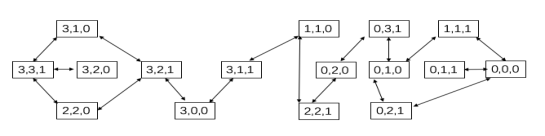
\includegraphics[width=\columnwidth]{fig1}
\end{center}

\end{itemize}

\section{Problem 2}
\begin{itemize}
	\item a). If all costs is 1, the cheapest solution is exactly the shallowest solution, i.e. $g(n)=depth(n)$. So uniform-cost search will become bread-first search.
	\item b). For best-first search, if $f(n)={\color{red}-}depth(n)$, then it will choose the deepest from frontier first and become depth-first search
	\item c). If the heuristic function of $\text{A}^*$  is $h(n)=0$, then it will become uniform-cost search. 
\end{itemize}

\section{Problem 3}
\begin{description}
	\item[a).] branching factor $b=4$.
	\item[b).] Since a step means $|x|$ or $|y|$ increase by 1, the final state satisfies $|x|+|y|=k \wedge |x|\le k \wedge |y| \le k$, which has $4k$ distinct states.
	\item[c).] Notation: frontier = set of nodes in frontier; |frontier| = number of nodes in frontier;   Acc. |frontier| = number of nodes expanded. The ${\color{red}-1}$ in tableau shows that  I think the destination node will be 'unfortunately' evaluated at the last among the nodes with the same depth, do not need to be expand (just evaluate/test). 
	
	\begin{tabular}{llll}
		\toprule
		depth & frontier & |frontier| & Acc. |frontier|\\
		\midrule 
		$d=0$ & $\{(0,0)\}$ & 1 & $1{\color{red}-1}$ \\
		$d=1$&$\{(0,1),(1,0),(-1,0),(0,-1)\}$&4&$5-1$\\
		$d=2$&   $\{(-1,1),(1,1),(0,0),(0,2),...,...,...\}$&16&$21-1$\\
		...&...&...&\\
		$d=k$&...&$4^k$&$(\sum_{n=0}^{k} 4^k) -1$\\
		\bottomrule
	\end{tabular}

	Therefore, Acc. |frontier|$=-1+\sum_{n=0}^{k} 4^k={(4^{k+1}-4)}/{3}={(4^{x+y+1}-4)}/{3}$
	
	\item[d).] Similarly, 
	
	\begin{tabular}{llll}
		\toprule
		depth & frontier & |frontier| & Acc. |frontier|\\
		\midrule 
		$d=0$ &$\{(0,0)\}$ & 1 & $1-1$ \\
		$d=1$&$\{(0,1),(1,0),(-1,0),(0,-1)\}$&4&$5-1$\\
		$d=2$&   $\{(x,y) \in \mathbb{R}^2; |x|+|y|=2\wedge |x|\le 2 \wedge |y|\le 2\}$&8&$13-1$\\
		...&...&...&\\
		$d=k$&$\{(x,y)\in \mathbb{R}^2; |x|+|y|=k\wedge |x|\le k \wedge |y|\le k\}$&$4k$&$-1+\sum_{n=0}^{k} 4k$\\
		\bottomrule
	\end{tabular}

	Therefore, Acc. |frontier|$=-1+\sum_{n=0}^{k} 4k=2k(k+1)=2(x+y)(x+y+1)$

	\item[e).] Yes, $h(n)=h^*(n)$ in this case and is admissible.
	\item[f).]  $\text{A}^*$ will search the nodes 'towards' destination, i.e. $\{(a,b)\in \mathbb{R}^2; 0\le a \le x \wedge 0 \le b \le y \}$. Totally, $(x+1)(y+1)-1$
	\item[g).] Yes, $h(n) \le h^*(n)$, since some links are removed.
	\item[h).] No,  $\exists n, h(n) > h^*(n)$, if current node n is  one of the ends of the added link.
	
\end{description}
%\begin{tabular}{|c|c|}
%	\hline 
%	&  \\ 
%	\hline 
%	&  \\ 
%	\hline 
%\end{tabular} 
\section{Problem 4}

\begin{center}
	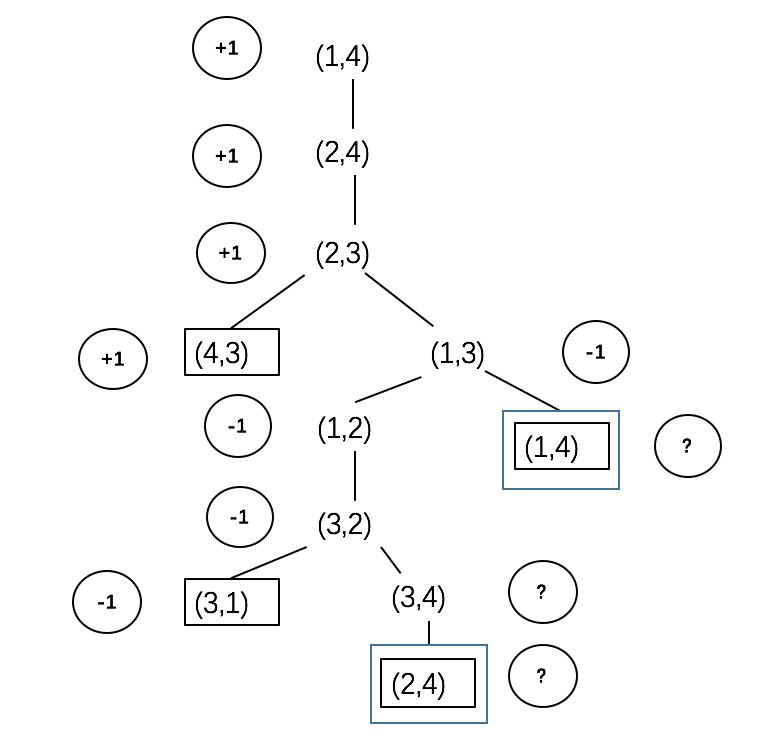
\includegraphics[width=.45\columnwidth]{fig2} \qquad 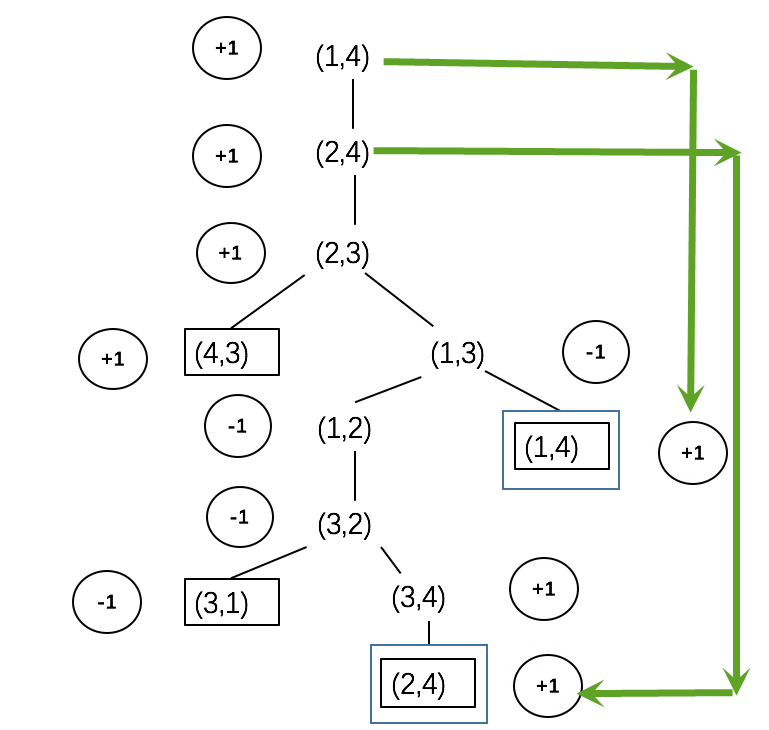
\includegraphics[width=.45\columnwidth]{fig3} \\
	\textbf{Left}: figure a for problem a. \  \textbf{Right}: figure b for problem b with backed-up values.
\end{center}

\begin{description}
	\item[b.] Ref. to fig. b. Use back-up, we can get optimal value of all the parent nodes. As for "?" values, we copy the value from visited node. It is right because for player A, $max(+1,?) = +1$; for player B $min(-1,?)=-1$ and thus we can prune the infinite branch. 
	\item[c.] Minmax algorithm fails because it use deep-first tree search and can go into infinite loop. The modified algorithm in \textit{b.} can not always give optimal decision for all games with loop. For example, if this 4-square game becomes a $2 \times 2$ matrix game, initialled as \begin{tabular}{|c|c|}
		\hline 
		A &  \\ 
		\hline 
		& B \\ 
		\hline 
	\end{tabular} , and we define
	\begin{center}
		

	\begin{tabular}{cc}
		\toprule
		A reaching & getting value of  \\ \midrule
		(0,0) & 1\\ 
		(0,1) & 2\\
		(1,0) & 3\\ 
		(1,1) & 4 \\ \bottomrule 
	\end{tabular}
	\end{center}
	 and B of the opposite value -1,-2,-3,-4. 
	 
	 Then we cannot decide the value of $max(+1,?)$, $max(+2,?)$, $min(-1,?)$ and so on and especially $min({\color{red}?},{\color{red}?})$ and $max({\color{red}?},{\color{red}?})$. Therefore, just to copy from appeared value will fail. 
	\item[d.] First consider n is odd. \begin{Proposition}
		If n is odd, then there exists a optimal strategy for B to win. 
	\end{Proposition}
	
	\begin{proof}
		
		\textbf{1).} For  n = 3, B will definitely win.
		
		\textbf{2).} Assume n-2 is odd, and there exists a optimal strategy for B to win.
		
		\textbf{3).} For n > 3, after first round, $(S_A,S_B)=(2,n-1)$, the size of square is n-2.
		According to \textit{2)}, there exists a strategy, s.t. $S_B=2 \wedge S_A\le n-2$ after the round of B. Next round of A, $S_A\le n-1$ then next round of B, B can choose move left (s.t. $S_B=1$) as its strategy and win. By induction, B will win when n is odd.
	\end{proof}
	
\end{description}
Similarly, if n is even, then there exists a optimal strategy for A to win. 
\section{Problem 5}
\begin{description}
	\item[a.] Up Triangle means max player, and Down Triangle means min player. Note that circle  means \textit{stochastic} strategy set. Use back-up, we get
	
	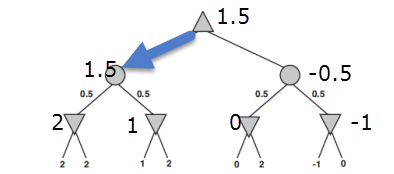
\includegraphics[width=.5\columnwidth]{fig4}
	\item[b.] Given leaves 1-6, we need to evaluate $x_7$ and $x_8$. If $\min(x_7,x_8)>3$ then the best move for max player won't be left. Given leaves 1-7, we do not need to evaluate $x_8$. $0.5\min(-1,x_8)+0.5*0\le -0.5$, the optimal move for max player keeps left.
	\item[c.] The value range for left-hand chance node: $[0,2]$
	\item[d.] After evaluating $x_5$ the value range for right-hand chance node is [-2,0], definitely smaller than 1.5. Thus $x_6,x_7,x_8$ can be pruned. 
	
	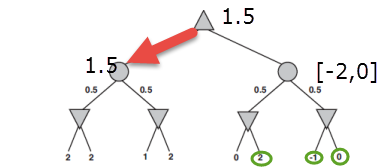
\includegraphics[width=.5\columnwidth]{fig5}
\end{description}


%\begin{thebibliography}{99}
%\bibitem{1} Silver, David, et al. "Mastering the game of Go with deep neural networks and tree search." Nature 529.7587 (2016): 484-489.
%Publishing Company , 1984-1986.
%\bibitem{2} \url{https://www.quora.com/Are-neural-networks-the-future-of-AI}
%\bibitem{3} \url{https://youtu.be/yCALyQRN3hw?list=PLqYmG7hTraZA7v9Hpbps0QNmJC4L1NE3S&t=11434}
%
%\end{thebibliography}	
	
\end{document}
